\documentclass[11pt]{article}

\usepackage[margin=1in]{geometry}
\usepackage{url}
\usepackage[separate-uncertainty, multi-part-units=single]{siunitx}
\usepackage{booktabs}
\usepackage{microtype}
\usepackage{graphicx}
\usepackage{multicol} \raggedcolumns
\usepackage{placeins}
\usepackage{caption}

\usepackage{hyperref}

\title{Evaluation of two methods for estimating Amazon Web Services cluster costs}
\author{Trevor K. McAllister-Day}

\begin{document}
	
	\maketitle
	
	\begin{multicols}{2}
		
		\section{Introduction}
		
		This is a comparison of two utilities for estimating the price of spinning up an Amazon Web Services (AWS) cluster. The first is Trevor's \texttt{price.sh}, written primarily in Python and Bash, and Tara's \texttt{get-spot-estimate}, written in R.
		
		Both are available on GitHub at \url{https://github.com/IBIC/AWS-Estimator.git}.
		
		Analysis was done with \texttt{compare-RP.R}, also available on GitHub.
		
		\section{Usage}
		
		Both the Python and the R implementations share the same basic functionality and features. The purpose of both is to take the estimated length of a single job (in hours) and the number of jobs, and create the cluster configuration that will be the cheapest. 
		
		Also available is a flag that allows searching of GPU-enabled instances (the g2 class).
		
		\section{Benchmarking}
		
		On the whole, the Python version is much faster than the R version. The Python version takes \SI{2.34\pm0.41}{\second} on average, and the R version \SI{208.10\pm10.90}{\second} (\SI{3.4683\pm0.1818}{\minute}). See \autoref{table:times}.		
		
		This provides an obvious advantage to the Python version when evaluating multiple configurations, however four minutes is not an overwhelming amount of time to wait for a single estimation.
		
		Every time it runs, the R program downloads a CSV file tabulating the most recent costs for each instance type, contributing to its increased execution time. 
		
	\end{multicols}
	
	\begin{table}[h]
		\centering
		\begin{tabular}{lrr}
			\toprule
			Program & Time (s) & N \\
			\midrule
			Python 	& \num{2.34\pm0.41}	& 20 \\
			R		& \num{208.10\pm10.90}	& 10 \\
			\bottomrule
		\end{tabular}
		\caption{Average execution times}
		\label{table:times}
	\end{table}
	
	\begin{multicols}{2}
		
		\section{Consistency}
		
		To compare the variance between the Python and R versions, I ran both \num{e5} times, looping over \numrange{1}{100} \si{\hour} and \numrange{1}{100} jobs, providing cost estimates in dollars for each permutation.
		
		While running the Python version took roughly \SI{6.5}{\hour}, running the R version was scheduled to take almost \SI{500}{\hour}. As it happens, the R run was interrupted by a failure of the IBIC cooling system, reaching only \num{827} time points.		
		However, this was enough to draw some conclusions and notice interesting patterns.
		
		On average, over the \num{827} available time points, there was no significant different between price estimations between the two programs ($p=.825$).
		
		The absolute average difference between program estimations was \SI{0.01478\pm0.01929}[\$]{}. In all comparisons, the Python estimation was greater than the R estimation.
		
		As a percentage of the total estimation, no difference between programs exceeded \SI{5}{\percent}, with the majority (\SI{97}{\percent}) of estimations within \SI{1.5}{\percent} of each other (see \autoref{fig:percent}). Average deviation was \SI{0.7515\pm.6313}{\percent}. 
		
	\end{multicols}
	
	\begin{figure}[h]
		\centering
		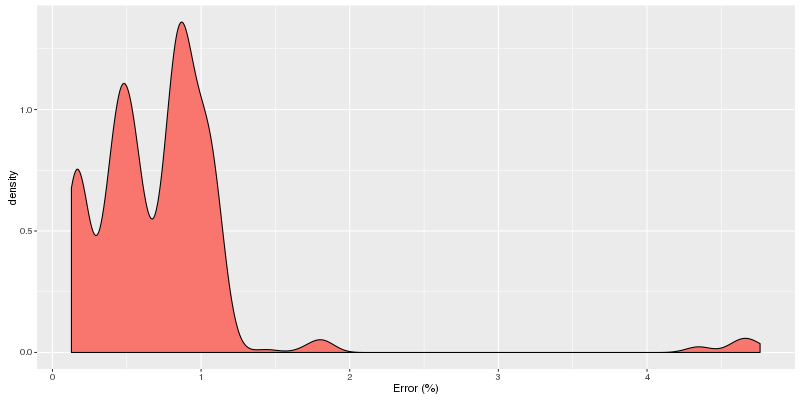
\includegraphics[width=0.7\textwidth]{error_percent}
		\caption{Distribution of percent errors}
		\label{fig:percent}
	\end{figure}
	
	\begin{multicols}{2}
		
		The far right hand end of \autoref{fig:percent} comprises 16 time points (\SI{2}{\percent} of the total) that occur when the number of jobs is equal to \num{63} or \num{64}. 
		
		This phenomenon occurs at every hour, up to \num{8} (the maximum number of hours completed up to the failure of the R benchmarking).		
		This effect can perhaps be more easily seen in \autoref{fig:bulges}, which also shows percent error increases with number of hours ($p<.001$). There is no main effect of number on percent error ($p=.064$).
		
		While the effect is minor, as can be seen in \autoref{fig:linear-comparison}, this effect is the result of decreased estimations by the R program.
		
		I was unable to replicate the effect in single repetitions of the R program.
				
	\end{multicols}
	
	\begin{minipage}{0.49\textwidth}
		\centering
		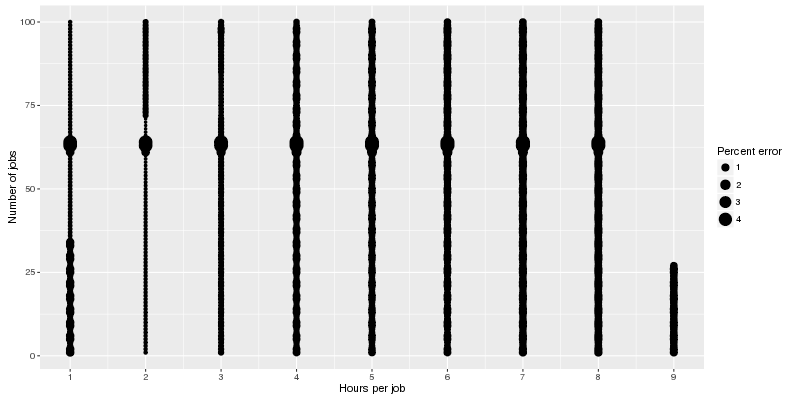
\includegraphics[width=\textwidth]{bulges}
		\captionof{figure}{Percent error by hour and number of jobs}
		\label{fig:bulges}
	\end{minipage}	
	\begin{minipage}{0.49\textwidth}
		\centering
		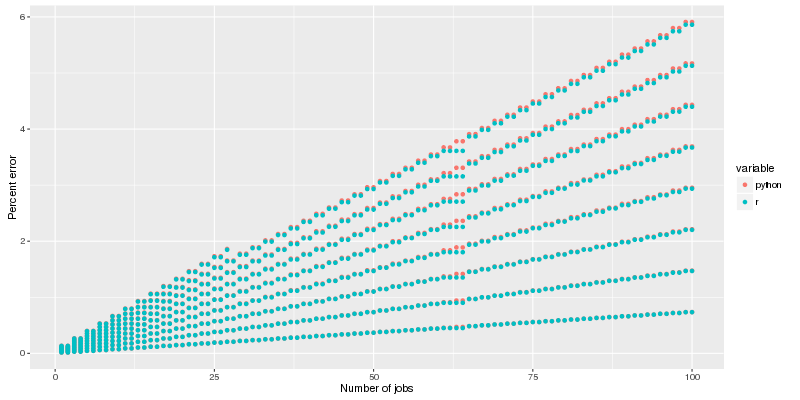
\includegraphics[width=\textwidth]{bad-r}
		\captionof{figure}{Estimate comparison}
		\label{fig:linear-comparison}
	\end{minipage}
	
	\FloatBarrier
	
	\begin{multicols}{2}
		
		\section{Conclusions}
		
		Both programs are functional and competent estimators of the cost to run a batch of jobs on an AWS cluster, and find nearly identical results.
		
		I recommend adding no more \SI{5}{\percent} to either estimator's results, as that accommodates even the most extreme errors the programs make. However, both programs will continue reporting their base calculations, and leave any price-buffering to the user, in order to be as transparent as possible.
		
	\end{multicols}
	
	
\end{document}